\documentclass[twoside]{book}

% Packages required by doxygen
\usepackage{fixltx2e}
\usepackage{calc}
\usepackage{doxygen}
\usepackage[export]{adjustbox} % also loads graphicx
\usepackage{graphicx}
\usepackage[utf8]{inputenc}
\usepackage{makeidx}
\usepackage{multicol}
\usepackage{multirow}
\PassOptionsToPackage{warn}{textcomp}
\usepackage{textcomp}
\usepackage[nointegrals]{wasysym}
\usepackage[table]{xcolor}

% Font selection
\usepackage[T1]{fontenc}
\usepackage[scaled=.90]{helvet}
\usepackage{courier}
\usepackage{amssymb}
\usepackage{sectsty}
\renewcommand{\familydefault}{\sfdefault}
\allsectionsfont{%
  \fontseries{bc}\selectfont%
  \color{darkgray}%
}
\renewcommand{\DoxyLabelFont}{%
  \fontseries{bc}\selectfont%
  \color{darkgray}%
}
\newcommand{\+}{\discretionary{\mbox{\scriptsize$\hookleftarrow$}}{}{}}

% Page & text layout
\usepackage{geometry}
\geometry{%
  a4paper,%
  top=2.5cm,%
  bottom=2.5cm,%
  left=2.5cm,%
  right=2.5cm%
}
\tolerance=750
\hfuzz=15pt
\hbadness=750
\setlength{\emergencystretch}{15pt}
\setlength{\parindent}{0cm}
\setlength{\parskip}{3ex plus 2ex minus 2ex}
\makeatletter
\renewcommand{\paragraph}{%
  \@startsection{paragraph}{4}{0ex}{-1.0ex}{1.0ex}{%
    \normalfont\normalsize\bfseries\SS@parafont%
  }%
}
\renewcommand{\subparagraph}{%
  \@startsection{subparagraph}{5}{0ex}{-1.0ex}{1.0ex}{%
    \normalfont\normalsize\bfseries\SS@subparafont%
  }%
}
\makeatother

% Headers & footers
\usepackage{fancyhdr}
\pagestyle{fancyplain}
\fancyhead[LE]{\fancyplain{}{\bfseries\thepage}}
\fancyhead[CE]{\fancyplain{}{}}
\fancyhead[RE]{\fancyplain{}{\bfseries\leftmark}}
\fancyhead[LO]{\fancyplain{}{\bfseries\rightmark}}
\fancyhead[CO]{\fancyplain{}{}}
\fancyhead[RO]{\fancyplain{}{\bfseries\thepage}}
\fancyfoot[LE]{\fancyplain{}{}}
\fancyfoot[CE]{\fancyplain{}{}}
\fancyfoot[RE]{\fancyplain{}{\bfseries\scriptsize Generated by Doxygen }}
\fancyfoot[LO]{\fancyplain{}{\bfseries\scriptsize Generated by Doxygen }}
\fancyfoot[CO]{\fancyplain{}{}}
\fancyfoot[RO]{\fancyplain{}{}}
\renewcommand{\footrulewidth}{0.4pt}
\renewcommand{\chaptermark}[1]{%
  \markboth{#1}{}%
}
\renewcommand{\sectionmark}[1]{%
  \markright{\thesection\ #1}%
}

% Indices & bibliography
\usepackage{natbib}
\usepackage[titles]{tocloft}
\setcounter{tocdepth}{3}
\setcounter{secnumdepth}{5}
\makeindex

% Hyperlinks (required, but should be loaded last)
\usepackage{ifpdf}
\ifpdf
  \usepackage[pdftex,pagebackref=true]{hyperref}
\else
  \usepackage[ps2pdf,pagebackref=true]{hyperref}
\fi
\hypersetup{%
  colorlinks=true,%
  linkcolor=blue,%
  citecolor=blue,%
  unicode%
}

% Custom commands
\newcommand{\clearemptydoublepage}{%
  \newpage{\pagestyle{empty}\cleardoublepage}%
}

\usepackage{caption}
\captionsetup{labelsep=space,justification=centering,font={bf},singlelinecheck=off,skip=4pt,position=top}

%===== C O N T E N T S =====

\begin{document}

% Titlepage & ToC
\hypersetup{pageanchor=false,
             bookmarksnumbered=true,
             pdfencoding=unicode
            }
\pagenumbering{roman}
\begin{titlepage}
\vspace*{7cm}
\begin{center}%
{\Large My Project }\\
\vspace*{1cm}
{\large Generated by Doxygen 1.8.11}\\
\end{center}
\end{titlepage}
\clearemptydoublepage
\tableofcontents
\clearemptydoublepage
\pagenumbering{arabic}
\hypersetup{pageanchor=true}

%--- Begin generated contents ---
\chapter{Class Index}
\section{Class List}
Here are the classes, structs, unions and interfaces with brief descriptions\+:\begin{DoxyCompactList}
\item\contentsline{section}{\hyperlink{structnode}{node} }{\pageref{structnode}}{}
\item\contentsline{section}{\hyperlink{structnode1}{node1} }{\pageref{structnode1}}{}
\item\contentsline{section}{\hyperlink{structnode__info}{node\+\_\+info} }{\pageref{structnode__info}}{}
\end{DoxyCompactList}

\chapter{File Index}
\section{File List}
Here is a list of all files with brief descriptions\+:\begin{DoxyCompactList}
\item\contentsline{section}{\hyperlink{Lab1_8c}{Lab1.\+c} }{\pageref{Lab1_8c}}{}
\end{DoxyCompactList}

\chapter{Class Documentation}
\hypertarget{classTime}{}\section{Time Class Reference}
\label{classTime}\index{Time@{Time}}


{\ttfamily \#include $<$Time.\+h$>$}

\subsection*{Public Member Functions}
\begin{DoxyCompactItemize}
\item 
\hyperlink{classTime_a0fc29d4a1be77a0f9fe1cd28c1d34958}{Time} (int h=0, int m=0, int s=0)
\item 
int \hyperlink{classTime_a4e9d93c2aaaac84b0a49f44184968860}{get\+Hour} () const 
\item 
void \hyperlink{classTime_a79e74e17893cf244e1318ceb9b1c7f32}{set\+Hour} (int h)
\item 
int \hyperlink{classTime_a6ccac73be7aacc12410cea6b3d216357}{get\+Minute} () const 
\item 
void \hyperlink{classTime_a35779c16a9db3499a27eccd58793f3b5}{set\+Minute} (int m)
\item 
int \hyperlink{classTime_adc2217366bfc4bb39eb547982747b6da}{get\+Second} () const 
\item 
void \hyperlink{classTime_a0528cf12858546b60ebb33fdcbc3fca2}{set\+Second} (int s)
\item 
void \hyperlink{classTime_ae05f94882a72debabb02e0889054d89a}{set\+Time} (int h, int m, int s)
\item 
void \hyperlink{classTime_acd9b7522e50fc667d81468219c5756e8}{print} () const 
\item 
void \hyperlink{classTime_a888a02dc15e919c5bafc4dcc95f093b7}{next\+Second} ()
\end{DoxyCompactItemize}
\subsection*{Private Attributes}
\begin{DoxyCompactItemize}
\item 
int \hyperlink{classTime_a497d35aa44ea40706dbab08f7a31d069}{hour}
\item 
int \hyperlink{classTime_a6c2e13147da34803a9784aa2b8bf8da8}{minute}
\item 
int \hyperlink{classTime_a63c9e64c7b453e10ba0f7f28bfedbcbf}{second}
\end{DoxyCompactItemize}


\subsection{Constructor \& Destructor Documentation}
\index{Time@{Time}!Time@{Time}}
\index{Time@{Time}!Time@{Time}}
\subsubsection[{\texorpdfstring{Time(int h=0, int m=0, int s=0)}{Time(int h=0, int m=0, int s=0)}}]{\setlength{\rightskip}{0pt plus 5cm}Time\+::\+Time (
\begin{DoxyParamCaption}
\item[{int}]{h = {\ttfamily 0}, }
\item[{int}]{m = {\ttfamily 0}, }
\item[{int}]{s = {\ttfamily 0}}
\end{DoxyParamCaption}
)}\hypertarget{classTime_a0fc29d4a1be77a0f9fe1cd28c1d34958}{}\label{classTime_a0fc29d4a1be77a0f9fe1cd28c1d34958}

\begin{DoxyCode}
8                               \{
9    \hyperlink{classTime_a497d35aa44ea40706dbab08f7a31d069}{hour} = h;
10    \hyperlink{classTime_a6c2e13147da34803a9784aa2b8bf8da8}{minute} = m;
11    \hyperlink{classTime_a63c9e64c7b453e10ba0f7f28bfedbcbf}{second} = s;
12 \}
\end{DoxyCode}


\subsection{Member Function Documentation}
\index{Time@{Time}!get\+Hour@{get\+Hour}}
\index{get\+Hour@{get\+Hour}!Time@{Time}}
\subsubsection[{\texorpdfstring{get\+Hour() const }{getHour() const }}]{\setlength{\rightskip}{0pt plus 5cm}int Time\+::get\+Hour (
\begin{DoxyParamCaption}
{}
\end{DoxyParamCaption}
) const}\hypertarget{classTime_a4e9d93c2aaaac84b0a49f44184968860}{}\label{classTime_a4e9d93c2aaaac84b0a49f44184968860}

\begin{DoxyCode}
15                         \{
16    \textcolor{keywordflow}{return} \hyperlink{classTime_a497d35aa44ea40706dbab08f7a31d069}{hour};
17 \}
\end{DoxyCode}
\index{Time@{Time}!get\+Minute@{get\+Minute}}
\index{get\+Minute@{get\+Minute}!Time@{Time}}
\subsubsection[{\texorpdfstring{get\+Minute() const }{getMinute() const }}]{\setlength{\rightskip}{0pt plus 5cm}int Time\+::get\+Minute (
\begin{DoxyParamCaption}
{}
\end{DoxyParamCaption}
) const}\hypertarget{classTime_a6ccac73be7aacc12410cea6b3d216357}{}\label{classTime_a6ccac73be7aacc12410cea6b3d216357}

\begin{DoxyCode}
25                           \{
26    \textcolor{keywordflow}{return} \hyperlink{classTime_a6c2e13147da34803a9784aa2b8bf8da8}{minute};
27 \}
\end{DoxyCode}
\index{Time@{Time}!get\+Second@{get\+Second}}
\index{get\+Second@{get\+Second}!Time@{Time}}
\subsubsection[{\texorpdfstring{get\+Second() const }{getSecond() const }}]{\setlength{\rightskip}{0pt plus 5cm}int Time\+::get\+Second (
\begin{DoxyParamCaption}
{}
\end{DoxyParamCaption}
) const}\hypertarget{classTime_adc2217366bfc4bb39eb547982747b6da}{}\label{classTime_adc2217366bfc4bb39eb547982747b6da}

\begin{DoxyCode}
35                           \{
36    \textcolor{keywordflow}{return} \hyperlink{classTime_a63c9e64c7b453e10ba0f7f28bfedbcbf}{second};
37 \}
\end{DoxyCode}
\index{Time@{Time}!next\+Second@{next\+Second}}
\index{next\+Second@{next\+Second}!Time@{Time}}
\subsubsection[{\texorpdfstring{next\+Second()}{nextSecond()}}]{\setlength{\rightskip}{0pt plus 5cm}void Time\+::next\+Second (
\begin{DoxyParamCaption}
{}
\end{DoxyParamCaption}
)}\hypertarget{classTime_a888a02dc15e919c5bafc4dcc95f093b7}{}\label{classTime_a888a02dc15e919c5bafc4dcc95f093b7}

\begin{DoxyCode}
60                       \{
61    ++\hyperlink{classTime_a63c9e64c7b453e10ba0f7f28bfedbcbf}{second};
62    \textcolor{keywordflow}{if} (\hyperlink{classTime_a63c9e64c7b453e10ba0f7f28bfedbcbf}{second} >= 60) \{
63       \hyperlink{classTime_a0528cf12858546b60ebb33fdcbc3fca2}{setSecond}(0);
64       \hyperlink{classTime_a35779c16a9db3499a27eccd58793f3b5}{setMinute}(++\hyperlink{classTime_a6c2e13147da34803a9784aa2b8bf8da8}{minute});
65    \}
66    \textcolor{keywordflow}{if} (\hyperlink{classTime_a6c2e13147da34803a9784aa2b8bf8da8}{minute} >= 60) \{
67       \hyperlink{classTime_a35779c16a9db3499a27eccd58793f3b5}{setMinute}(0);
68       \hyperlink{classTime_a79e74e17893cf244e1318ceb9b1c7f32}{setHour}(++\hyperlink{classTime_a497d35aa44ea40706dbab08f7a31d069}{hour});
69    \}
70    \textcolor{keywordflow}{if} (\hyperlink{classTime_a497d35aa44ea40706dbab08f7a31d069}{hour} >= 24) \{
71       \hyperlink{classTime_a79e74e17893cf244e1318ceb9b1c7f32}{setHour}(0);
72    \}
73 \}\end{DoxyCode}
\index{Time@{Time}!print@{print}}
\index{print@{print}!Time@{Time}}
\subsubsection[{\texorpdfstring{print() const }{print() const }}]{\setlength{\rightskip}{0pt plus 5cm}void Time\+::print (
\begin{DoxyParamCaption}
{}
\end{DoxyParamCaption}
) const}\hypertarget{classTime_acd9b7522e50fc667d81468219c5756e8}{}\label{classTime_acd9b7522e50fc667d81468219c5756e8}

\begin{DoxyCode}
52                        \{
53    cout << setfill(\textcolor{charliteral}{'0'});    \textcolor{comment}{// zero-filled, need <iomanip>, sticky}
54    cout << setw(2) << \hyperlink{classTime_a497d35aa44ea40706dbab08f7a31d069}{hour}  \textcolor{comment}{// set width to 2 spaces, need <iomanip>, non-sticky}
55         << \textcolor{stringliteral}{":"} << setw(2) << \hyperlink{classTime_a6c2e13147da34803a9784aa2b8bf8da8}{minute}
56         << \textcolor{stringliteral}{":"} << setw(2) << \hyperlink{classTime_a63c9e64c7b453e10ba0f7f28bfedbcbf}{second} << endl;
57 \}
\end{DoxyCode}
\index{Time@{Time}!set\+Hour@{set\+Hour}}
\index{set\+Hour@{set\+Hour}!Time@{Time}}
\subsubsection[{\texorpdfstring{set\+Hour(int h)}{setHour(int h)}}]{\setlength{\rightskip}{0pt plus 5cm}void Time\+::set\+Hour (
\begin{DoxyParamCaption}
\item[{int}]{h}
\end{DoxyParamCaption}
)}\hypertarget{classTime_a79e74e17893cf244e1318ceb9b1c7f32}{}\label{classTime_a79e74e17893cf244e1318ceb9b1c7f32}

\begin{DoxyCode}
20                         \{
21    \hyperlink{classTime_a497d35aa44ea40706dbab08f7a31d069}{hour} = h;
22 \}
\end{DoxyCode}
\index{Time@{Time}!set\+Minute@{set\+Minute}}
\index{set\+Minute@{set\+Minute}!Time@{Time}}
\subsubsection[{\texorpdfstring{set\+Minute(int m)}{setMinute(int m)}}]{\setlength{\rightskip}{0pt plus 5cm}void Time\+::set\+Minute (
\begin{DoxyParamCaption}
\item[{int}]{m}
\end{DoxyParamCaption}
)}\hypertarget{classTime_a35779c16a9db3499a27eccd58793f3b5}{}\label{classTime_a35779c16a9db3499a27eccd58793f3b5}

\begin{DoxyCode}
30                           \{
31    \hyperlink{classTime_a6c2e13147da34803a9784aa2b8bf8da8}{minute} = m;
32 \}
\end{DoxyCode}
\index{Time@{Time}!set\+Second@{set\+Second}}
\index{set\+Second@{set\+Second}!Time@{Time}}
\subsubsection[{\texorpdfstring{set\+Second(int s)}{setSecond(int s)}}]{\setlength{\rightskip}{0pt plus 5cm}void Time\+::set\+Second (
\begin{DoxyParamCaption}
\item[{int}]{s}
\end{DoxyParamCaption}
)}\hypertarget{classTime_a0528cf12858546b60ebb33fdcbc3fca2}{}\label{classTime_a0528cf12858546b60ebb33fdcbc3fca2}

\begin{DoxyCode}
40                           \{
41    \hyperlink{classTime_a63c9e64c7b453e10ba0f7f28bfedbcbf}{second} = s;
42 \}
\end{DoxyCode}
\index{Time@{Time}!set\+Time@{set\+Time}}
\index{set\+Time@{set\+Time}!Time@{Time}}
\subsubsection[{\texorpdfstring{set\+Time(int h, int m, int s)}{setTime(int h, int m, int s)}}]{\setlength{\rightskip}{0pt plus 5cm}void Time\+::set\+Time (
\begin{DoxyParamCaption}
\item[{int}]{h, }
\item[{int}]{m, }
\item[{int}]{s}
\end{DoxyParamCaption}
)}\hypertarget{classTime_ae05f94882a72debabb02e0889054d89a}{}\label{classTime_ae05f94882a72debabb02e0889054d89a}

\begin{DoxyCode}
45                                       \{
46    \hyperlink{classTime_a79e74e17893cf244e1318ceb9b1c7f32}{setHour}(h);
47    \hyperlink{classTime_a35779c16a9db3499a27eccd58793f3b5}{setMinute}(m);
48    \hyperlink{classTime_a0528cf12858546b60ebb33fdcbc3fca2}{setSecond}(s);
49 \}
\end{DoxyCode}


\subsection{Member Data Documentation}
\index{Time@{Time}!hour@{hour}}
\index{hour@{hour}!Time@{Time}}
\subsubsection[{\texorpdfstring{hour}{hour}}]{\setlength{\rightskip}{0pt plus 5cm}int Time\+::hour\hspace{0.3cm}{\ttfamily [private]}}\hypertarget{classTime_a497d35aa44ea40706dbab08f7a31d069}{}\label{classTime_a497d35aa44ea40706dbab08f7a31d069}
\index{Time@{Time}!minute@{minute}}
\index{minute@{minute}!Time@{Time}}
\subsubsection[{\texorpdfstring{minute}{minute}}]{\setlength{\rightskip}{0pt plus 5cm}int Time\+::minute\hspace{0.3cm}{\ttfamily [private]}}\hypertarget{classTime_a6c2e13147da34803a9784aa2b8bf8da8}{}\label{classTime_a6c2e13147da34803a9784aa2b8bf8da8}
\index{Time@{Time}!second@{second}}
\index{second@{second}!Time@{Time}}
\subsubsection[{\texorpdfstring{second}{second}}]{\setlength{\rightskip}{0pt plus 5cm}int Time\+::second\hspace{0.3cm}{\ttfamily [private]}}\hypertarget{classTime_a63c9e64c7b453e10ba0f7f28bfedbcbf}{}\label{classTime_a63c9e64c7b453e10ba0f7f28bfedbcbf}


The documentation for this class was generated from the following files\+:\begin{DoxyCompactItemize}
\item 
\hyperlink{Time_8h}{Time.\+h}\item 
\hyperlink{Time_8cpp}{Time.\+cpp}\end{DoxyCompactItemize}

\chapter{File Documentation}
\hypertarget{Time_8cpp}{}\section{Time.\+cpp File Reference}
\label{Time_8cpp}\index{Time.\+cpp@{Time.\+cpp}}
{\ttfamily \#include $<$iostream$>$}\\*
{\ttfamily \#include $<$iomanip$>$}\\*
{\ttfamily \#include $<$stdexcept$>$}\\*
{\ttfamily \#include \char`\"{}Time.\+h\char`\"{}}\\*
Include dependency graph for Time.\+cpp\+:
\nopagebreak
\begin{figure}[H]
\begin{center}
\leavevmode
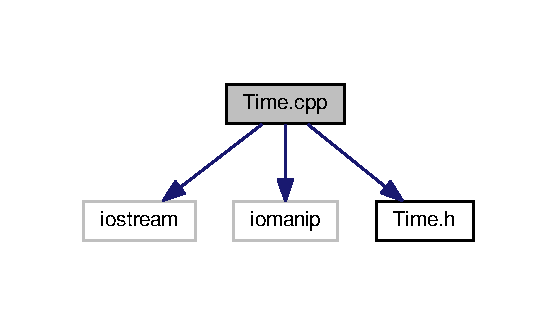
\includegraphics[width=345pt]{Time_8cpp__incl}
\end{center}
\end{figure}

\hypertarget{Time_8h}{}\section{Time.\+h File Reference}
\label{Time_8h}\index{Time.\+h@{Time.\+h}}
This graph shows which files directly or indirectly include this file\+:
\nopagebreak
\begin{figure}[H]
\begin{center}
\leavevmode
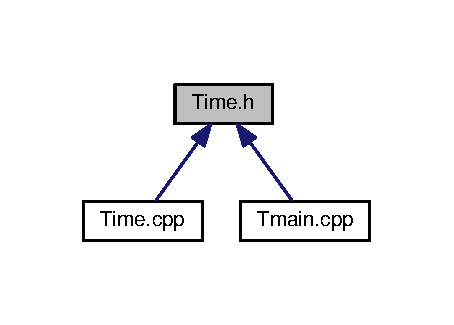
\includegraphics[width=218pt]{Time_8h__dep__incl}
\end{center}
\end{figure}
\subsection*{Classes}
\begin{DoxyCompactItemize}
\item 
class \hyperlink{classTime}{Time}
\end{DoxyCompactItemize}

\hypertarget{Tmain_8cpp}{}\section{Tmain.\+cpp File Reference}
\label{Tmain_8cpp}\index{Tmain.\+cpp@{Tmain.\+cpp}}
{\ttfamily \#include $<$iostream$>$}\\*
{\ttfamily \#include \char`\"{}Time.\+h\char`\"{}}\\*
Include dependency graph for Tmain.\+cpp\+:
\nopagebreak
\begin{figure}[H]
\begin{center}
\leavevmode
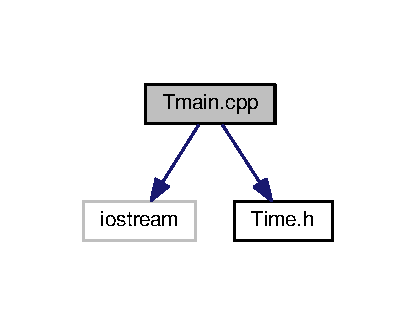
\includegraphics[width=200pt]{Tmain_8cpp__incl}
\end{center}
\end{figure}
\subsection*{Functions}
\begin{DoxyCompactItemize}
\item 
int \hyperlink{Tmain_8cpp_ae66f6b31b5ad750f1fe042a706a4e3d4}{main} ()
\end{DoxyCompactItemize}


\subsection{Function Documentation}
\index{Tmain.\+cpp@{Tmain.\+cpp}!main@{main}}
\index{main@{main}!Tmain.\+cpp@{Tmain.\+cpp}}
\subsubsection[{\texorpdfstring{main()}{main()}}]{\setlength{\rightskip}{0pt plus 5cm}int main (
\begin{DoxyParamCaption}
{}
\end{DoxyParamCaption}
)}\hypertarget{Tmain_8cpp_ae66f6b31b5ad750f1fe042a706a4e3d4}{}\label{Tmain_8cpp_ae66f6b31b5ad750f1fe042a706a4e3d4}

\begin{DoxyCode}
6            \{
7    \textcolor{comment}{// Ordinary object}
8    \hyperlink{classTime}{Time} t1(1, 2, 3);
9    t1.print();  \textcolor{comment}{// 01:02:03}
10  
11    \textcolor{comment}{// Object pointer}
12    \hyperlink{classTime}{Time}* ptrT1 = &t1;
13    (*ptrT1).\hyperlink{classTime_acd9b7522e50fc667d81468219c5756e8}{print}(); \textcolor{comment}{// 01:02:03}
14    ptrT1->\hyperlink{classTime_acd9b7522e50fc667d81468219c5756e8}{print}();   \textcolor{comment}{// 01:02:03}
15       \textcolor{comment}{// anObjectPtr->member is the same as (*anObjectPtr).member}
16  
17    \textcolor{comment}{// Object reference}
18    \hyperlink{classTime}{Time}& refT1 = t1; \textcolor{comment}{// refT1 is an alias to t1}
19    refT1.\hyperlink{classTime_acd9b7522e50fc667d81468219c5756e8}{print}();    \textcolor{comment}{// 01:02:03}
20  
21    \textcolor{comment}{// Dynamic allocation}
22    \hyperlink{classTime}{Time}* ptrT2 = \textcolor{keyword}{new} \hyperlink{classTime}{Time}(4, 5, 6); \textcolor{comment}{// allocate dynamically}
23    ptrT2->\hyperlink{classTime_acd9b7522e50fc667d81468219c5756e8}{print}(); \textcolor{comment}{// 04:05:06}
24    \textcolor{keyword}{delete} ptrT2;   \textcolor{comment}{// deallocate}
25  
26    \textcolor{comment}{// Object Array}
27    \hyperlink{classTime}{Time} tArray1[2];    \textcolor{comment}{// tArray1 is an array of Time with 2 elements}
28                        \textcolor{comment}{// Use default constructor for all elements}
29    tArray1[0].\hyperlink{classTime_acd9b7522e50fc667d81468219c5756e8}{print}();  \textcolor{comment}{// 00:00:00}
30    tArray1[1].\hyperlink{classTime_acd9b7522e50fc667d81468219c5756e8}{print}();  \textcolor{comment}{// 00:00:00}
31  
32    \hyperlink{classTime}{Time} tArray2[2] = \{\hyperlink{classTime}{Time}(7, 8, 9), \hyperlink{classTime}{Time}(10)\}; \textcolor{comment}{// Invoke constructor}
33    tArray2[0].\hyperlink{classTime_acd9b7522e50fc667d81468219c5756e8}{print}();  \textcolor{comment}{// 07:08:09}
34    tArray2[1].\hyperlink{classTime_acd9b7522e50fc667d81468219c5756e8}{print}();  \textcolor{comment}{// 10:00:00}
35  
36    \hyperlink{classTime}{Time}* ptrTArray3 = \textcolor{keyword}{new} \hyperlink{classTime}{Time}[2]; \textcolor{comment}{// ptrTArray3 is a pointer to Time}
37             \textcolor{comment}{// Dynamically allocate an array of Time with 2 elements via new[]}
38    ptrTArray3[0].\hyperlink{classTime_acd9b7522e50fc667d81468219c5756e8}{print}();  \textcolor{comment}{// 00:00:00}
39    ptrTArray3[1].\hyperlink{classTime_acd9b7522e50fc667d81468219c5756e8}{print}();  \textcolor{comment}{// 00:00:00}
40    \textcolor{keyword}{delete}[] ptrTArray3;    \textcolor{comment}{// Deallocate dynamic array via delete[]}
41  
42    \textcolor{comment}{// C++11 syntax, compile with -std=c++0x}
43    \hyperlink{classTime}{Time}* ptrTArray4 = \textcolor{keyword}{new} \hyperlink{classTime}{Time}[2] \{\hyperlink{classTime}{Time}(11, 12, 13), \hyperlink{classTime}{Time}(14)\}; \textcolor{comment}{// Invoke constructor}
44    ptrTArray4->\hyperlink{classTime_acd9b7522e50fc667d81468219c5756e8}{print}();        \textcolor{comment}{// 11:12:13}
45    (ptrTArray4 + 1)->print();  \textcolor{comment}{// 14:00:00}
46    \textcolor{keyword}{delete}[] ptrTArray4;
47 \}\end{DoxyCode}


Here is the call graph for this function\+:
\nopagebreak
\begin{figure}[H]
\begin{center}
\leavevmode
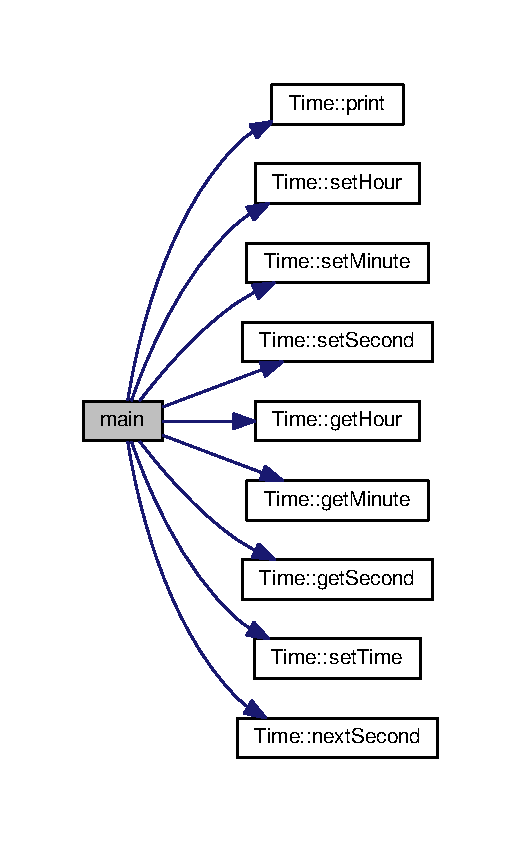
\includegraphics[width=217pt]{Tmain_8cpp_ae66f6b31b5ad750f1fe042a706a4e3d4_cgraph}
\end{center}
\end{figure}



%--- End generated contents ---

% Index
\backmatter
\newpage
\phantomsection
\clearemptydoublepage
\addcontentsline{toc}{chapter}{Index}
\printindex

\end{document}
